\section{Evaluation Design}\label{sec:evaluation}
We ask four questions. \textbf{RQ1:} Can a source-conditioned schedule return genuine failure feedback with fewer executed tests and lower measured process time? \textbf{RQ2:} Does a frontier-aware tree improve measured certificate traffic after charging initialization? \textbf{RQ3:} Do missing, stale, conflicting, or adversarially incomplete records ever obtain a local pass? \textbf{RQ4:} Which costs and negative results limit practical value?

\subsection{Executable subjects and scope}
We use exact local source copies of NetworkX~\cite{networkx}, Toolz~\cite{toolz}, and Future Code Control v1.2.0. The first two are upstream libraries with their unmodified existing tests. The third is the uploaded agent-runtime prototype, not an independent industrial deployment. Source copies and licenses are included in the artifact. A public benchmark download was unavailable because container DNS resolution failed; we did not substitute invented external-benchmark results.

The frozen scopes contain 170 NetworkX tests for components, traversal, and unweighted/generic shortest paths; 148 Toolz tests for iterable, functional, dictionary, recipe, curried, and utility behavior; and 138 Future Code core tests for contracts, state, coordination, and hierarchy. All scoped baselines passed. Separately, the original Future Code full suite passed all 263 tests. The mutation study does not claim to rerun that full 263-test scope on every changed candidate. An initially considered SymPy scope was excluded before mutation outcomes because its upstream test configuration required an unavailable dependency; the replacement with Toolz is recorded in the contract.

\begin{table}[t]
\centering\small
\caption{Executable subjects. Mutation cells report rejected / surviving / unresolved cases, not autonomous repairs. A surviving mutant is not a proof of semantic equivalence.}\label{tab:cohort}
\begin{tabular}{@{}lrrrr@{}}
\toprule
Subject & Tests & Training & Development & Confirmation\\
\midrule
NetworkX & 170 & 11/5/0 & 9/5/1 & 5/4/0\\
Toolz & 148 & 9/2/0 & 8/2/0 & 6/0/0\\
Future Code & 138 & 8/10/0 & 10/8/0 & 12/6/0\\
\bottomrule
\end{tabular}
\end{table}


\subsection{Predefined interventions and disclosed development decisions}
For each of 17 predefined source files, we select up to six nonoverlapping AST sites by a fixed seeded hash. Operators alter relational boundaries, arithmetic operators, Boolean constants, or negation. Only the selected expression span changes; the surrounding file is not reformatted. Selected sites alternate between training and development. This yields 45 training and 43 development cases. We retain surviving mutants, timeouts, and collection failures rather than replacing them with easier-to-detect faults. A surviving mutant means only that the scoped tests did not reject it.

After the development outcomes revealed conditional-tree overfitting, we fixed pooled-frontier layout as the revised default and froze 33 additional intervention sites with a new seed. These sites do not overlap any training or development mutation span, including nested expressions. They span 11 source files; some files had too few unused sites. The original 45 training cases, ranker, and serialized plans remain fixed. Confirmation outcomes do not refit them. Model-plan hashes and the freeze timestamp precede all confirmation executions. This is a local registered experimental contract, not a claim of third-party preregistration.

Every full-oracle execution runs in a fresh private source copy. We check the intended mutant hash and store pytest phase records. A completed oracle must have the exact registry and a final pass/fail outcome for every obligation. Incomplete or timed-out attempts remain unknown and are excluded only from metrics requiring a complete finite oracle; their counts remain visible. Full-oracle runs use four worker processes for throughput. Their durations are not used as controlled latency measurements because of resource contention.

\subsection{Baselines and measurements}
The prioritization baselines are default collection order, shortest-first, file-call coverage first, global empirical fault-set cover, and source-conditioned fault-set cover. All are full permutations. We replay each ordering against the complete outcome vector to count executed tests to first failure; replayed phase time is explicitly not wall-clock latency.

For actual timing, the development cohort consists of the first eight predefined development IDs per project. After retaining one incomplete oracle as unknown, 23 eligible snapshots are executed with four orderings and three repetitions, for 276 fresh subprocess runs. The confirmation timing cohort is the first four confirmation IDs per project, with default, call-profile, and source-conditioned orderings and three repetitions. The exact eligible count and observed agreement are given below. Within each repetition, candidate blocks and ordering labels are deterministically randomized. Repetitions are not treated as independent source mutations.

Timing includes process startup, imports, pytest collection, test execution, evidence writing, and order planning. It excludes source copying, offline tree fitting, and certificate replay. A separate strict-wrapper smoke test includes copying, source hashing, and certificate generation. We report per-candidate medians of three repetitions, then aggregate those paired values. Variance from startup and scheduling is real and must not be hidden behind a test-count ratio.

Tree baselines use the same conditional schedule and outcome vectors: (a) a compact bottom-up eight-ary fixed tree; (b) the old invalidation-only exact optimizer, which sees every interval active under strict whole-snapshot invalidation; (c) a pooled-frontier tree; and (d) per-source frontier trees. All trees preserve the same registry order and 3072-byte cap. The invalidation-only optimizer is an objective ablation, not the strongest practical baseline; the compact fixed tree is essential. We run the trusted kernel for each evaluated tree and sum actual serialized packet lengths, including the first full construction. This is a measured protocol replay over real outcomes, not live network transmission.

\paragraph{Uncertainty and estimands.}
For paired comparisons, the primary reduction is $100(1-\sum_i y_i/\sum_i x_i)$, where $x_i$ and $y_i$ are baseline and candidate measurements on the same mutation. Confidence intervals use a seeded paired cluster bootstrap, resampling source-file clusters within each project; timing first reduces repeated runs to per-mutation medians. These intervals are conditional on three chosen projects and the intervention design. They do not establish generalization to a population of repositories. We also report project-level values, absolute seconds/bytes, and unfavorable comparisons.

\section{Results}
\subsection{Failure feedback and actual latency}
\begin{table}[t]
\centering\small
\caption{Mean executed tests to first failure, among oracle-rejected candidates only. Counts are schedule replay over complete real test outcomes. Successful and unresolved candidates are not in this denominator.}\label{tab:checks}
\begin{tabular}{@{}llrrrrr@{}}
\toprule
Subject & Split & Failures & Default & Calls & Global & Cond.\\
\midrule
NetworkX & Dev. & 9 & 79.4 & 5.8 & 40.8 & 6.0\\
Toolz & Dev. & 8 & 67.9 & 25.9 & 71.2 & 21.5\\
Future Code & Dev. & 10 & 67.4 & 26.6 & 14.0 & 5.1\\
NetworkX & Confirm. & 5 & 79.2 & 6.0 & 9.2 & 1.6\\
Toolz & Confirm. & 6 & 47.3 & 35.5 & 57.3 & 20.0\\
Future Code & Confirm. & 12 & 79.5 & 29.9 & 34.2 & 15.8\\
\bottomrule
\end{tabular}
\end{table}

\begin{table}[t]
\centering\small
\caption{Measured process seconds: means of per-candidate medians from three repetitions. Each cohort includes both rejected and surviving candidates. Includes startup/collection/evidence writing; excludes snapshot copying, offline fitting and certificate replay.}\label{tab:time}
\begin{tabular}{@{}llrrrrr@{}}
\toprule
Subject & Split & Cases & Default & Calls & Global & Cond.\\
\midrule
NetworkX & Dev. & 7 & 2.832 & 2.805 & 2.872 & 2.841\\
Toolz & Dev. & 8 & 1.410 & 1.412 & 1.449 & 1.371\\
Future Code & Dev. & 8 & 2.073 & 1.835 & 1.819 & 1.870\\
NetworkX & Confirm. & 4 & 2.851 & 2.912 & -- & 2.813\\
Toolz & Confirm. & 4 & 1.371 & 1.408 & -- & 1.402\\
Future Code & Confirm. & 4 & 1.808 & 1.716 & -- & 1.726\\
\bottomrule
\end{tabular}
\end{table}

On the fresh confirmation failures, the conditional policy executes a mean of 13.78 checks before rejection, versus 26.17 for the call-profile baseline: 47.34\% fewer, with a source-cluster 95\% interval [19.26, 77.46]. This is evidence of earlier failure in the test sequence, not automatically faster feedback in seconds. Across the confirmation timing cohort, mean per-candidate median process times are 2.010 seconds (default), 2.012 seconds (call-profile), and 1.980 seconds (conditional). The paired reduction versus call-profile is 1.58\% with interval [0.62, 2.01], compared with 1.48\% versus default with interval [-1.06, 5.70]. The development cohort also shows no consistent advantage over call-profile (-0.45\%; interval [-1.31, 0.36]). Startup and collection can dominate these short scopes. We therefore do not claim a large or consistently reproduced wall-clock improvement over the stronger ordering baseline.

\begin{figure}[t]
\centering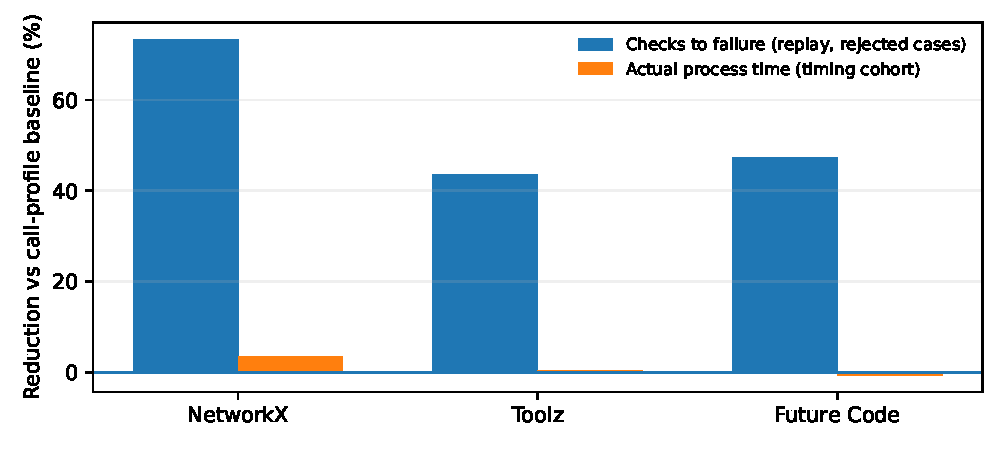
\includegraphics[width=.90\linewidth]{generated/feedback_tradeoff.pdf}
\caption{Sequence efficiency is not wall-clock acceleration. Confirmation check-count reductions use all oracle-rejected cases; timing reductions use the separately frozen timing cohort. The two denominators are intentionally labeled and must not be equated.}
\label{fig:feedback}
\end{figure}

\subsection{Certificate traffic and the negative specialization result}
\begin{table}[t]
\centering\small
\caption{Mean actual aggregation traffic in KiB per completed candidate, including full initial construction. The same conditional schedule is used for every tree; logs, raw evidence and transport framing are excluded.}\label{tab:traffic}
\begin{tabular}{@{}llrrrrr@{}}
\toprule
Subject & Split & Cases & Fixed-8 & Inval. & Pooled & Per-source\\
\midrule
NetworkX & Dev. & 14 & 288.7 & 606.2 & 267.7 & 414.6\\
Toolz & Dev. & 10 & 198.9 & 357.9 & 183.9 & 243.6\\
Future Code & Dev. & 18 & 248.9 & 480.8 & 213.9 & 207.8\\
NetworkX & Confirm. & 9 & 327.9 & 709.1 & 302.2 & 362.2\\
Toolz & Confirm. & 6 & 120.4 & 170.5 & 113.7 & 132.7\\
Future Code & Confirm. & 18 & 225.9 & 444.7 & 196.6 & 191.4\\
\bottomrule
\end{tabular}
\end{table}

The fresh confirmation result is a reduction from 234.5 to 210.3 KiB per candidate, or 10.33\% with source-cluster interval [8.86, 11.66]. The development reduction is 10.22\%. Per-source trees are not the selected default: they cost 26.93\% more than pooled frontiers on development. On confirmation, pooled frontiers use 7.48\% fewer bytes than per-source layouts. Table~\ref{tab:traffic} retains project-level counterexamples, including the Future Code cases where per-source layout is smaller. Initialization is charged on every candidate and no favorable steady-state-only accounting is used.


The invalidation-only objective can produce a deep tree with low one-time construction cost but expensive repeated progress updates. This is not an optimizer bug: it is the wrong objective for that trace. Conversely, a compact fixed hierarchy is a strong baseline, and data-dependent layout is not uniformly superior on every candidate. Lower aggregate bytes do not imply faster execution or higher repair quality.

\subsection{Soundness and integrity checks}
All 384 actual timing executions agree with their complete scoped oracle verdicts; none of these timing runs timed out. All 300 certificate-layout decisions on 75 evaluable development/confirmation candidates agree with their source oracle. The sole incomplete development oracle remains unresolved; it is not converted to pass. In the controlled edge-pruning replay, the unsafe reuse comparator would accept 8 of 23 confirmation candidates rejected by the full oracle. The unpruned call-profile reuse comparator has no observed false pass in this cohort; the pruning result is a deliberate stress test, not a claim that its natural graph failed. Strict complete-registry authorization does not rely on either graph.

The protocol tests exercise complete coverage, missing leaves, stale bindings, same-content and ABA epoch changes, contradictory same-epoch evidence, idempotent retries, invalid layouts, tampered displays, and local concurrent submissions. Exhaustive enumeration of small binary trees checks the compiler independently of the DP recurrence. A separate auditor reads stored trees and outcomes and recomputes packet costs without importing the optimizer or the producer's pricing helpers. It also checks site disjointness, source hashes, registry equality, timing-record identities, and observed verdict agreement.

We additionally replay a deliberately unsafe comparator that assumes a previous pass can be reused for every test outside an observed call graph. Its edge-pruning ablation removes three quarters of file--test edges by an outcome-independent hash. Any false pass in that ablation demonstrates the danger of allowing incomplete learned relationships to authorize acceptance. It is not a measurement of NameRTS, and it does not estimate an attack rate in production. The strict protocol never converts omitted checks into pass evidence.

\subsection{Overhead, batching, and practical boundaries}
The pooled compiler takes 0.177--0.302 seconds per project in the width-eight sensitivity run. A synthetic complete-pass kernel-only run with the same registries and five repetitions has a median of 14.2--19.0 ms; this measures the Python protocol, not project tests. The real-project wrapper smoke adds 0.301--0.517 seconds beyond its pytest process for copying, identities, contract checks and certificates. These integrity costs are material relative to the small observed ordering-time differences. We do not claim that the wrapper makes bare pytest faster end to end.

The empirical priority needs historic complete outcomes; producing these through deliberate fault injection costs real testing time. A production deployment should normally reuse approved development/repair traces or justify a bounded offline intervention budget, rather than continuously mutating a production checkout. Tree fitting is offline and should be amortized. If startup dominates the suite or few candidates fail, the benefit of reordering can be small. Successful strict candidates still execute the full registry.
